\documentclass[prl,amsmath,amssymb, twocolumn, showpacs]{revtex4-1}
%showpacs, twocolumn
\usepackage{dcolumn}
\usepackage{bm}
\usepackage{graphicx}
\usepackage{hyperref}
\usepackage{mathptmx}
\usepackage{subfigure}
\usepackage[utf8]{inputenc}
\usepackage{bbold}
\usepackage{color}
\newcommand{\david}[1]{{\color{red} #1}}
\newcommand{\ata}[1]{{\color{blue} #1}}




\newcommand{\pp}{p_{al}}

\makeatletter


\begin{document}

\title{Efficient algorithm for the periodic Lorentz gas in 2 and 3 dimensions}
\author{Atahualpa S.~Kraemer}
\email{ata.kraemer@gmail.com}
\affiliation{Institut für Theoretische Physik II - Soft Matter
Heinrich-Heine-Universität Düsseldorf
Building 25.32
Room O2.56
Universitätsstrasse 1
D-40225 Düsseldorf, Germany}

\author{Nikolay Kryukov}
\email{kryukov@ciencias.unam.mx}

\author{David P.~Sanders}
\email{dpsanders@ciencias.unam.mx}
\affiliation{Departamento de F\'isica, Facultad de Ciencias, Universidad Nacional
Aut\'onoma de M\'exico,
Ciudad Universitaria, M\'exico D.F.\ 04510, Mexico
}

\date{\today}
\begin{abstract}

We present an efficient algorithm to calculate collisions for a periodic Lorentz gas in 2 and 3 dimensions, using continued fractions. The method works very well in the 2-dimensional case, obtaining the exact disc with which a particle will collide at each step, instead of using periodic boundary conditions. However, the 3D case obtains these coordinates only with a probability $\pp$ which depends on the size of the obstacles as $\pp= 1-(16-\sqrt{128}-\frac{4}{3} \pi) r^3 \sim 1-0.5 r^3$. This 3D algorithm is generalizable to higher dimensions; however, the efficiency of the method becomes worse. 
\end{abstract}

\maketitle

\section{Introduction}



Lorentz gases are probably the simplest systems that present deterministic chaos \cite{cvitanovic1992investigation}, and probably one of the most popular models in statistical mechanics and nonlinear dynamics which is known as Sinai billiard when the scatterers are periodic \cite{bunimovich1981statistical}. This model consists of an array of scatterers (usually spheres), placed in the vertices of a grid, and particles which move freely until they encounter obstacles where they experience inelastic collisions. 

This kind of systems can have different configuration of the scatterers, as for example, random lattices \cite{latz1997lyapunov,dellago1997lyapunov, van1998chaotic} or quasiperiodic systems \cite{kraemer2013embedding,wennberg2012free}. However, because of the simplicity, the periodic case has been widely studied (see e.g. \cite{bunimovich1981statistical,bleher1992statistical, chernov1994statistical, gilbert2011diffusive}), but there are still many open questions \cite{gilbert2009persistence,marklof2011periodic,nandori2012tail, dettmann2012new}. Many of the results obtained theoretically for these gases are in the limit where obstacles are very small, i.e. the Boltzmann--Grads limit \cite{caglioti2003distribution, golse2012recent,boca2007distribution,golse2006periodic,caglioti2008boltzmann,caglioti2010boltzmann, golse2000distribution,marklof2008kinetic, bourgain1998distribution}. 

Usually, in this case, simulations are made in a single cell, with periodic boundary conditions (or reflecting in the borders) with an obstacle in the middle of the cell\cite{sanders2008normal,  sanders2005fine}. However, this implies that the program must check each time when the particle crosses a border, whether it will collide with the obstacle in the cell, or it will move to the next cell. That implies solving at least two linear equations and one quadratic, then checking if the solution of the quadratic equation is real and finally taking the maximum value among the three (or two in case of the complex solution to the quadratic equation) results. If the obstacle is big enough, it is quite probable that the particle will collide each time it crosses the boundary. However, in the Boltzmann-Grads limit, this situation does not happen very often, and then the program loses much time checking when particles cross the boundary and if there is a collision with the obstacle even if there is not.

A suitable situation would be a formula to find the coordinates of the next obstacle giving the position and velocity of the particle. As we will see in section \ref{algorithm} this is indeed the first solution of the Diophantine inequality:

\begin{equation}
|\alpha q+b-p|\leq  \frac{v^2}{v_x} r
\end{equation}

where $r$ is the radius of the obstacles, $q$ and $p$ are integer variables, and $\alpha$ and $b$ are two real numbers related to the position $\vec{x}$ and velocity $\vec{v}$ of the particle. But this inequality is closely related to the best rational approximant to an irrational number for the case $b=0$ and the solutions can be obtained by the continued fraction algorithm. 

Apparently the algorithm for this, using continued fractions, was developed before \cite{zacherl1986power}. However, it was never published by their authors. Nevertheless, the continued fractions were used on several occasions to develop the theory about the free path distribution of the periodic Lorentz gas in the Boltzmann-Grads limit \cite{caglioti2003distribution, golse2012recent,boca2007distribution,golse2006periodic,caglioti2008boltzmann, caglioti2010boltzmann, golse2000distribution, bleher1992statistical,chernov1994statistical}, and relatively recently, Golse has developed an algorithm to coding particles trajectories by using the continued fraction algorithm, and the 3-length theorem \cite{golse2012recent}. However, this algorithm a priory works only if the particle leaves the surface of a disk. This restriction makes the algorithm not useful in other geometries as quasiperiodic arrays or two incommensurate overlapping arrays of square lattices and different shapes of obstacles, but those system may produce a number of surprising effects \cite{}.  On the other hand, because the way the algorithm is made (using the 3-length theorem and continued fraction algorithm), it is not possible to use it in higher dimensions, the fact that was noted by Golse, arguing that the one involving higher dimensions ''is a notoriously more difficult problem''.

\section{2D algorithm}
\label{algorithm}

The goal of the 2D algorithm is to calculate efficiently where the first collision of a particle will occur inside a square lattice. Without loss of generality, we will use the lattice formed by the integer coordinates in the 2D plane. Then, we want to calculate the minimal time $t>0$, such that $|\vec{c}-(\vec{x_0}+\vec{v_0}t)|=r$, where $r$ is the radius of the obstacle, $\vec{x_0}$ and $\vec{v_0}$ are the initial position and velocity of the particles, and $\vec{c}=(q,p)$ are the integer coordinates. In this case, the collision takes place at the point $\vec{x_0}+\vec{v_0}t$, with the center of the obstacle at $\vec{c}$. 

As the first improvement over the classical algorithm for the 2D case note that instead of finding the intersection between a line (corresponding to the trajectory of the particle, $y=\alpha x+b$) and a circle (corresponding to the obstacle $(x-q)^2+(y-p)^2=r^2$), we can solve the intersection between two lines: $y=\alpha x+b$ and $x=q$. As it is shown in figure \ref{fig:circle}, if $|\alpha q+b-p|=|b|<\delta=r/v_1$, then a collision will take place. Of course, this is true only if $v_1>0$ and $v_2>0$, but after each collision, we can always rotate or reflect the system (because of the symmetry) such that these conditions are satisfied. Even better, because of the periodic boundary conditions, we can always put $0 < b < 1$, then we only need to solve $b<\delta$, this already gives us a very powerful tool to calculate with which obstacle the particle will collide. 

Indeed, we do not need to apply periodic boundary conditions at every step, we only need to check 
\begin{equation}
|\{ \alpha  q_n \}+b -1|< \delta, 
\label{eq:master}
\end{equation}
where $\{ \cdot \}$ denotes the fractional part, and $q_n=q_{n-1}+1$, where $q_1$ is the $x$-coordinate of the closest obstacle to the particle at $t=0$. Then, the first $q_n$ that satisfies this inequality will be $q$. To calculate $p$, we can note that always $p=\lfloor \alpha q +b\rfloor$ or $p=\lfloor \alpha q +b\rfloor+1$

\begin{figure}
\centering
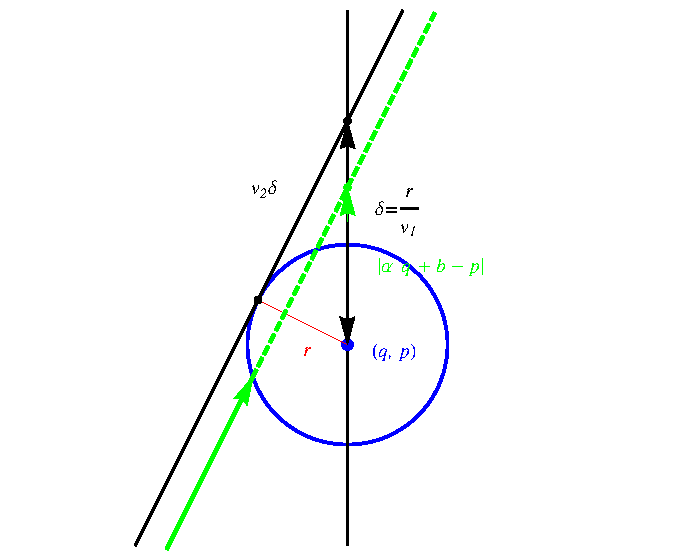
\includegraphics [width=240pt]{fig01.pdf}
\caption{Relation between the intersection of a line and a circle with integer coordinates and the intersection of the line with the x-axis}
\label{fig:circle}
\end{figure}


Now, to simplify even more the algorithm, consider the integer coordinates $(q_n, q_n)$ such that
\begin{equation}
|\alpha q_n -p_n + b|< \delta,
\label{eq:1}
\end{equation}
and for any pair of numbers $(i,j)$ such that $i<q_n$, then $|\alpha i -j+ b|> \delta$,  $q=q_n$, and $p=p_n$. 
 
But $|\alpha q_i - p_i + b|$ are the distances between the integer coordinates $(q_i, p_i)$ and the point $( q_i ,\alpha q_i + b)$, then, we would like a succession such that  
\begin{equation}
|\alpha q_i - p_i + b|<|\alpha q_{i-1} - p_{i-1} + b|
\label{eq:iteration}
\end{equation}
for every $i>1 \in   \mathbb{N}$. Also, the first pair of integer coordinates $q_0$ and $p_0$ should be $(0, 0)$ or $(0, 1)$, minimizing $|\alpha q_0 - p_0 + b|$, that is:

\begin{equation}
|\alpha q_1 -p_1 + b|< f(b) = \begin{cases} b &\mbox{if } b < 1/2 \\ 
1-b & \mbox{if } b > 1/2 \end{cases} 
\label{eq:prima}
\end{equation}

Note that $p_n= \lfloor \alpha q_n +b  \rfloor= \begin{cases} \lfloor \alpha q_n  \rfloor  &\mbox{if } b+\alpha q_n-\lfloor \alpha q_n  \rfloor < 1 \\ 
 \lfloor \alpha q_n  \rfloor+1  &\mbox{if } b+\alpha q_n-\lfloor \alpha q_n  \rfloor > 1 \end{cases}$ if $b<1/2$ or $p_n= \lfloor \alpha q_n +b  \rfloor+1= \begin{cases} \lfloor \alpha q_n  \rfloor+1  &\mbox{if } b+\alpha q_n-\lfloor \alpha q_n  \rfloor < 1 \\ 
 \lfloor \alpha q_n  \rfloor+2  &\mbox{if } b+\alpha q_n-\lfloor \alpha q_n  \rfloor > 1 \end{cases}$ if $b>1/2$, then, substituting the four cases form here in the two cases of equation \ref{eq:prima}, we obtain that indeed $p_1= \lfloor \alpha q_1  \rfloor+1$, and then,  iterating  equation \ref{eq:iteration} we obtain 

\begin{equation}
 p_n= \lfloor \alpha q_n  \rfloor+1.
\label{eq:hn}
\end{equation}
 
Mixing the inequality \ref{eq:1} and equation \ref{eq:hn}, we obtain again equation \ref{eq:master}. 

Thus, we have reduced the solution from two linear equations and one quadratic to one linear equation. Even more, now we do not check in every periodic cell, because if $\alpha >1$, for every $q_n$ we advance $\alpha$ cells. And we don't need to apply periodic boundary conditions until we reach the obstacle. 

\subsection{The Diophantine inequality: $|\alpha p - q|\leq \epsilon$}

Now, a better algorithm should find a way to find the set of $p_i$, such that inequality \ref{eq:iteration} keeps and there is not any integer $q$ such that there exists an $i$ such that $p_i<q<p_{i-1}$ and
$|\{ \alpha  q_i \}+b -1|<|\{ \alpha  q \}+b -1| <|\{ \alpha  q_{i-1} \}+b -1|$. 

In order to do this, we can use the continued fraction algorithm to obtain solutions to the inequality $|\alpha q - p|\leq \epsilon$. This algorithm already gives a succession of $(q_n,p_n)$ such that $|\alpha q_i - p_i|<|\alpha q_{i-1} - p_{i-1}|$ if $q_{i-1} <q_i$. So, if we turn our inequality \ref{eq:prima} into this other inequality, we will find our algorithm just by using the continued fraction algorithm.
Indeed, using equation \ref{eq:hn} and the inequality \ref{eq:prima}, we obtain $|\{ \alpha  q_1 \} -1|< \begin{cases} 2b &\mbox{if } b < 1/2 \\  2(1-b) & \mbox{if } b > 1/2 \end{cases} $, which is almost the continued fraction inequality, except that $p$ is always equal to $\lfloor \alpha q  \rfloor+1$. 

\begin{equation}
|\alpha  q-p|< \begin{cases} 2b &\mbox{if } b < 1/2 \\  2(1-b) & \mbox{if } b > 1/2 \end{cases}
\label{eq:master2}
\end{equation}

Then, we can apply the continued fraction algorithm to obtain $p$ and $q$ of inequality \ref{eq:master2}. If $\lfloor \alpha q  \rfloor+1$, then, we have found $(q_1,p_1)$ otherwise not, but we know that $p_1\geq p$, and $q_1 \geq q$ then we can just use $(q, p)$ even if they do not satisfy inequality \ref{eq:iteration}, then calculate the succession $b_i$ as $b_0=b$, $b_i=\{\alpha q_i+b\}$. If $b_n<\delta$ the algorithm stops, and the collision will take place with the obstacle centered at the coordinates $(q_n,p_n)$. 

\subsection{Explicit algorithm}

Now we have all the necessary tools to implement the complete algorithm step by step. The Julia language is used here.

Call \texttt{frac($\alpha, \epsilon$)} the function that obtains the first integers $(q,p)$, such that $|\alpha q-p|<\epsilon$ by using the continued fraction algorithm (see appendix). 

\begin{verbatim}
function frac(x, epsilon) 
   h1, h2 = 1, 0 
    k1, k2 = 0, 1 
    b = x 
   while abs(k1*x - h1) > epsilon 
       a = ifloor(b) 
       h1, h2 = a*h1 + h2, h1 
        k1, k2 = a*k1 + k2, k1 
       b = 1/(b - a) 
    end 
   return k1, h1 
end
\end{verbatim}


Now, define the function \texttt{eff(m, b, r)} as follows: 
\begin{verbatim}
function eff(m, b, r)
	kn = 0
    b1 = b
    epsilon = r*sqrt(m*m+1) 
    if(b < epsilon || 1 - b < epsilon)
        if b < BigFloat("0.5")
			(q, p) = frac(m, 2.*b)
		else
			(q, p) = frac(m, 2.*(1. - b))
		end
		b = mod(m*q + b, 1)
		kn += q
    end  
	while b > epsilon && 1 - b > epsilon
		if b < BigFloat("0.5")
			(q, p) = frac(m, 2.*b)
		else
			(q, p) = frac(m, 2.*(1. - b))
		end
		b = mod(m*q + b, 1)
		kn += q
	end
	q = kn
    p = int(m*q+b1)
    return [q, p]
end
\end{verbatim}

This function applies the continued fraction algorithm along with the inequality \ref{eq:master2} until the distance in the y-direction between the line and the integer coordinates $(q, p)$ is less than $\epsilon$. 

Then, the algorithm to localize the first obstacle, with which a particle with velocity $\vec{v}$ and position $\vec{x}$ will collide, is as follows (in pseudocode): 

\begin{verbatim}
if (v is in quadrant I) then     
   (q,p)=efficient_algorithm(m, b, delta)
   p=int(m*q)+1
else if (v is in quadrant II) then
   m=-m                               
   % reflect the system with 
   %respect to y-axis 
   (q,p)=efficient_algorithm(m, b, delta)
   p=int(m*q)+1
   m=-m                                
   % reflect the system with 
   %respect to y-axis
   q=-q                                
   % reflect the system with 
   %respect to y-axis
else if (v is in quadrant III) then
   b=1-b                              
   % reflect the system with 
   %respect to the origin
   (q,p)=efficient_algorithm(m, b, delta)
   b=1-b                              
   % reflect the system with 
   %respect to the origin
   p=-(int(m*q)+1)                               
   % reflect the system with 
   %respect to the origin
   q=-q                               
   % reflect the system with 
   %respect to the origin
else if (v is in quadrant IV) then
   b=1-b                              
   % reflect the system with 
   %respect to the x-axis
   m=-m                               
   % reflect the system with 
   %respect to the x-axis
   (q,p)=efficient_algorithm(m, b, delta)             
   b=1-b                              
   % reflect the system with 
   %respect to the x-axis
   m=-m                               
   % reflect the system with 
   %respect to the x-axis
   p=-(int(m*q)+1)                               
   % reflect the system with 
   %respect to the x-axis
endif
\end{verbatim}

Using the technique mentioned above, which, for the initial position $(0, b), 0 < b < 1$ and for any initial velocity returns the integer coordinates of the obstacle of the first collision, we make the function \texttt{Lorentz(x, v, r)} that calculates the first collision of the particle in the 2D plane. In order to calculate the exact collision point and the velocity after the collision, we need to use the classical collision functions \texttt{collision} and \texttt{velo\_col}.

The functions \texttt{frac}, \texttt{eff} and \texttt{Lorentz}, which comprise the implementation of the efficient algorithm, and the classical functions to calculate the trajectory, can be found in the module (LINK TO MODULE).


\section{3D case}

In the previous section we developed an algorithm to efficiently calculate the motion of particles in a 2-dimensional periodic Lorentz gas. However, the same ideas cannot be applied directly to a 3-dimensional case. In this section we will show how to use this method in higher dimensions, losing some efficiency.

\paragraph{3D algorithm} If we project a 3D cubic lattice onto the $xy$, $xz$ or $yz$ plane, we will obtain a periodic square lattice. Also, if we project a 3D line onto those planes, we will obtain a 2D line parametrized by a linear function of the time. 
Then we can apply the 2D algorithm onto the 3 projections, and take the maximum time $t$ among the 3 obtained times. We will call $s$ the distance covered by the particle in the maximum time $t$. If the obstacle coordinates are the same in the 3 planes, we will check if the particle collides with this obstacle; if not, we move the particle by the distance $s$, then we advance to the next cell, we apply periodic boundary conditions, and we use again the 2D continued fraction algorithm in the 3 projected planes. 

Using the 2D continued fraction algorithm in each of the 3 planes $xy$, $xz$ and $yz$ is equivalent to calculating a collision with a cylinder orthogonal to those planes. Then, taking only the solution where the particle collides in the 3 planes is equivalent to calculating the coordinates of the center of the intersection of the three orthogonal cylinders with the same radius. 
As Figure \ref{fig:collision} shows, even in the case when the 3 planes obtain the same coordinate of the obstacle, with this distance ($s$), the 3D algorithm will not always find the next collision because some trajectories will collide with the intersection of the three orthogonal cylinders but will not have a collision with the sphere. However, we can assure that the first collision will take place in a time longer or equal than the time $t$. Then, we can check if the collision takes place. If it happens, we calculate the collision by calculating the intersection between the sphere with radius $\delta$ and coordinates $\vec{h_{n}}$ where $\vec{h_{n}}$ are the 3 integers obtained with the 3D algorithm, and the line that describes the trajectory of the particle. If there is no collision, we move up to the next cell after the calculated distance, apply periodic boundary conditions, and apply again the 3D algorithm. 
\begin{figure}
\centering
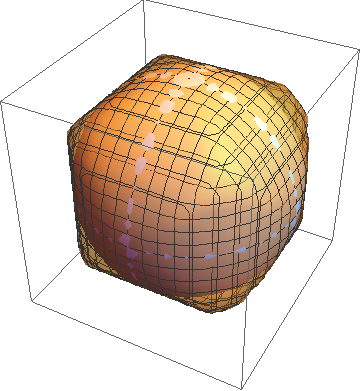
\includegraphics [width=240pt]{./region.png}
\caption{A sphere of radius $r$ embedded into the intersection of 3 orthogonal cylinders of the same radius. The volume where there is no sphere, but there is the intersection of the 3 cylinders, is the place where trajectories of particles can be considered as having collisions, when really they do not use the proposed algorithm in the 3D case.}
\label{fig:collision}
\end{figure}


Also, as Figure \ref{fig:collision} suggests, the difference $\pp$ between the real obstacle and the intersection of the cylinders is not large. This difference measures directly the probability that the 3D algorithm will find the next collision. In other words, the probability $\pp$ that the 3D algorithm will find the next collision is: 

\begin{equation}
\pp= 1-(16-\sqrt{128}-\frac{4}{3} \pi) r^3 \sim 1-0.5 r^3, 
\end{equation}
which is very small for small obstacles (for example, obstacles of radius $r=0.01$ will produce a probability $\pp \sim 0.999995$ that the algorithm will find the next collision). 

The 3D algorithm is realized by the above mentioned technique based on applying the 2D algorithm function \texttt{Lorentz} in the projections on the 3 planes and is in the function \texttt{Lorentz3D} in the module (LINK TO MODULE).


\section{Numerical measurements}

We measured the average time of the execution of the function finding the first collision starting from the initial point around the origin, depending on the radius of the obstacle, for both the classical and efficient algorithms.

\begin{figure}
\centering
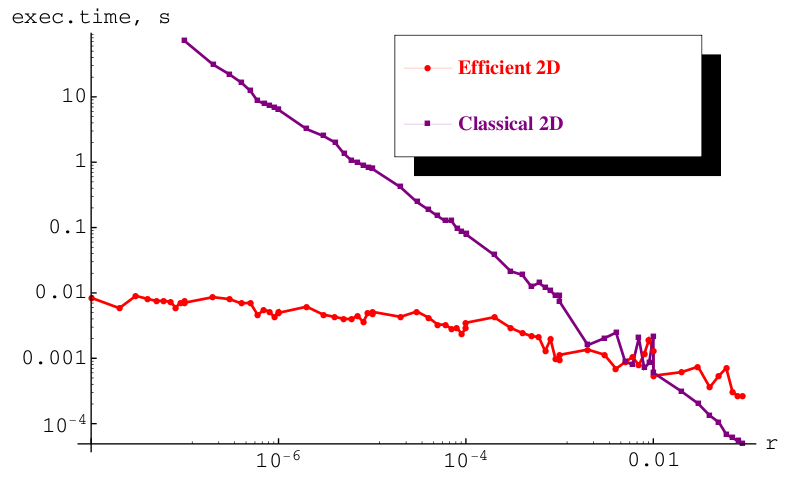
\includegraphics [width=260pt]{fig05.png}
\caption{Average execution time of finding the first collision in 2D Lorentz gas, for the classical and efficient allgorithms.}
\label{fig:fig05}
\end{figure}

\begin{figure}
\centering
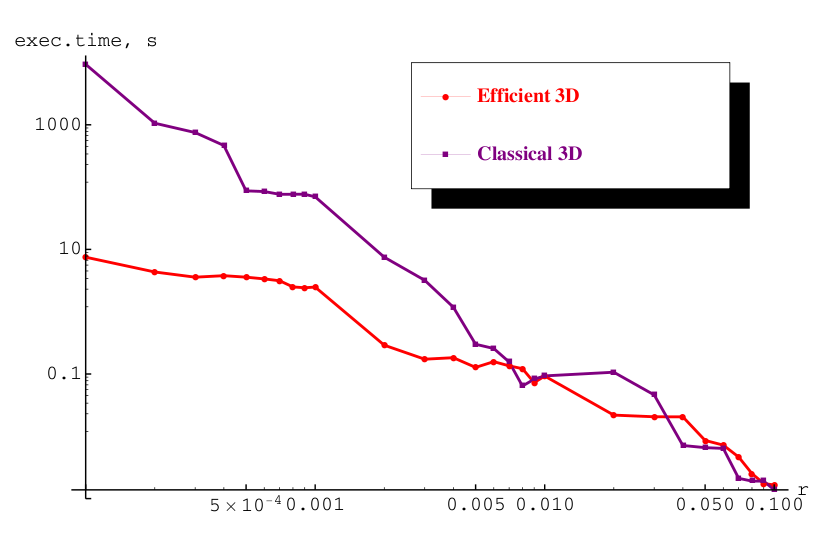
\includegraphics [width=260pt]{fig06.png}
\caption{Average execution time of finding the first collision in 2D Lorentz gas, for the classical and efficient allgorithms.}
\label{fig:fig06}
\end{figure}

Figures \ref{fig:fig05} and \ref{fig:fig06} show the results of this simulation for 2D and 3D versions. As we can see, the new algorithm is significantly more efficient for $r < 0.01$.





\section{Conclusions}  

We have presented an efficient algorithm to study periodic Lorentz gases in 2 and 3 dimensions when the obstacles are in the Boltzmann-Grad limit, i.e. when the obstacles are very small. 

\section{Acknowledgments}  
We thank ... ASK received support from the ERC Advanced Grant
INTERCOCOS (Grant No. 267499). and DPS received financial support from CONACYT Grant CB-101246 and DGAPA-UNAM PAPIIT Grants
IN116212 and IN117214.


\section{Appendix: Approximation of irrational numbers by rational}

In this section we will summarize some of the principal results about continued fractions that we will use in the algorithm. The demonstrations can be found in many books on number theory (see for example \cite{niven2008introduction}). The geometrical interpretation was also suggested before by many other authors (see, for example, \cite{nogueira1995three}). 

Let us define a continued fraction as follows:
A continued fraction is an expression obtained through an iterative process of representing a number $\alpha$ as the sum of its integer part $a_0$ and the reciprocal of another number $\alpha_1=\alpha-a_0$, then writing $\alpha_1$ as the sum of its integer part $a_1$ and the reciprocal of $\alpha_2=\alpha_1-a_1$, and so on. 
\begin{equation*}
  \alpha = a_0 + \frac{1}{\displaystyle a_1
          + \frac{1}{\displaystyle a_2
          + \frac{1}{\displaystyle a_3 + \dots}}}
\end{equation*}

This expression produces a succession of integer numbers $\lfloor \alpha \rfloor=a_0,\lfloor \alpha_1 \rfloor=a_1, \lfloor \alpha_2 \rfloor=a_2, \dots$. 
Then, we define inductively two successions of integers $\{ p_n\}$ and $\{ q_n\}$ in the following way:

\begin{alignat}{2}
p_{-2} = 0,  &\quad p_{-1} = 1,  &\quad p_i=a_i p_{i-1}+p_{i-2}
\label{eq:sucesion1}
\\ 
q_{-2} = 1,  &\quad q_{-1} = 0,  &\quad q_i=a_i q_{i-1}+q_{i-2} 
\label{eq:sucesion2}
\end{alignat}

With this succession we can approximate any irrational number $\alpha$ using the Hurwitz theorem:
\emph{For every irrational number $\alpha$ all the relative prime integers $p_n$, $q_n$ of the successions defined in equations \ref{eq:sucesion1} and \ref{eq:sucesion2} keep the formula:}
\begin{equation}
|\alpha- \frac{p_n}{q_n}|\leq  \frac{1}{{q_n}^2} 
\end{equation}


\bibliographystyle{apsrev}
\bibliography{Bib-alg}


\end{document}
